\documentclass[11pt]{article}

\usepackage[margin=1.15in]{geometry}
\usepackage{amsmath}
\usepackage{amssymb}
\usepackage{graphicx}
\usepackage{xcolor}
\usepackage{tikz}

% One symbol per object, as in notes/correlated_bias_prior_v2.
\newcommand{\Cov}{\mathsf{C}}
\newcommand{\T}{^{\mathsf{T}}}
\newcommand{\kmax}{k_{\rm max}}
\newcommand{\hMpc}{\,h/{\rm Mpc}}
\newcommand{\aunit}{\,h^{-2}\,{\rm Mpc}^2}
\newcommand{\bstwo}{b_{s^2}}
\newcommand{\SNz}{{\rm SN}_0}
\newcommand{\SNt}{{\rm SN}_2}
% The parameter-recovery statistic.  It has no name.
\newcommand{\chidof}{\sqrt{\langle\chi^2\rangle/n_{\rm dof}}}
% The matrices of the Fisher assembly, sans-serif as in the
% correlated-prior note, so that the derivative matrix D is not the
% growth factor D(z).
\newcommand{\mB}{\mathsf{B}}
\newcommand{\mM}{\mathsf{M}}
\newcommand{\mD}{\mathsf{D}}
\newcommand{\mG}{\mathsf{G}}
\newcommand{\nbase}{n_{\rm base}}
\newcommand{\npar}{n_{\rm par}}
% An underscore after which a long code name may break.
\newcommand{\us}{\_\allowbreak}

% Okabe-Ito colors of the schematic (no red or green).
\definecolor{okblue}{HTML}{0072B2}
\definecolor{okorange}{HTML}{E69F00}
\definecolor{oksky}{HTML}{56B4E9}

\title{Fisher forecasts from cached derivatives}
\date{November 2026}
\author{}

\emergencystretch=3em
% let the schematic share a page with text
\renewcommand{\topfraction}{0.85}
\renewcommand{\textfraction}{0.1}
\renewcommand{\floatpagefraction}{0.75}

\begin{document}

\begin{center}
  {\LARGE Fisher forecasts from cached derivatives\par}
  \vspace{0.4em}
  {\large How the derivatives are computed and stored, and why every\\
    FoM, error and shift is recomputed in seconds\par}
  \vspace{0.6em}
  {\large November 2026\par}
\end{center}
\vspace{1em}

\section{Summary}
\label{sec:summary}

\paragraph{The question.}
The project's Fisher notebooks report figures of merit (FoMs),
marginalized errors and parameter shifts for four bias variants, up to
four linear-bias priors, seven scale cuts and four bin layouts, under
dozens of assumed truths.  One likelihood evaluation runs CAMB and
CosmoLike's non-Limber projection of every thin bin, and the
derivatives of one layout took roughly $15$ to $45$ minutes during
development.  How, then, can a change of model, prior or scale cut cost
only seconds?

\paragraph{The answer.}
\begin{enumerate}
  \item A Fisher forecast linearizes the data vector around one point,
    so it needs the derivatives at that point and nothing else
    (Section~\ref{sec:linear}).
  \item For each layout the notebooks compute a fixed set of base
    columns once, the derivatives with respect to the cosmology, to
    four bias operators in every bin and to the terms linear in their
    amplitude, and cache them on disk (Section~\ref{sec:base}).
  \item A bias model is a fixed matrix $\mM$ that combines the base
    columns, $\mD = \mB\mM$, by the chain rule.  A new model is a new
    $\mM$ (Section~\ref{sec:models}).
  \item A scale cut keeps a subset of the rows, and each cut is reduced
    once to the matrix $\mG = \mB\T \Cov^{-1} \mB$, at most
    $645 \times 645$ (Section~\ref{sec:cuts}).  Every Fisher matrix is
    then $\mM\T \mG \mM$ plus priors, and every FoM, shift and
    $\langle\chi^2\rangle$ is a product of small matrices
    (Section~\ref{sec:downstream}).
  \item New likelihood evaluations are needed only for a term outside
    the base columns, a new fiducial point, or effects beyond first
    order (Section~\ref{sec:limits}).  Section~\ref{sec:usage} lists
    the cache files and what invalidates them.
\end{enumerate}

\paragraph{The setup.}
The data are the DESI band powers $C_\ell^{gg}$, the angular power
spectrum averaged in $53$ multipole bands, computed without the Limber
approximation for six tracer groups $g$ (BGS, LRG1, LRG2, LRG3, ELG1
and ELG2) on four layouts: bins of equal comoving width
$\Delta d_{\rm com} = 62$~Mpc, and bins of fixed redshift width
$\Delta z = 0.02$, $0.05$ and $0.2$.  Bin $i$ has mean redshift
$\bar{z}_i$, and $D(z)$ is the linear growth factor, $D(0) = 1$.  The
bias models A and B and the linear-bias priors are those of the
correlated-prior note, \texttt{notes/correlated\_bias\_prior\_v2}.

\section{Why derivatives at one point are enough}
\label{sec:linear}

Let $m(p)$ be the expected data vector at the parameters $p$, $p_0$ the
fiducial point and $\Cov$ the covariance of the data.  The vector $m$
has $n$ entries: the band powers of every bin's auto spectrum and of
every measured cross pair of bins, after $795$ entries that the data
format reserves for cosmic-shear blocks and that stay zero for DESI
alone.  Near $p_0$
\begin{equation}
  m(p) \;\simeq\; m(p_0) + \mD\,(p - p_0),
  \qquad
  \mD_{aj} = \frac{\partial m_a}{\partial p_j}\bigg|_{p_0} ,
  \label{eq:linearize}
\end{equation}
so a Gaussian likelihood becomes a Gaussian in $p$.  With Gaussian
priors of precision $F_{\rm prior}$, the posterior has the inverse
covariance
\begin{equation}
  F \;=\; \mD\T \Cov^{-1} \mD \;+\; F_{\rm prior} ,
  \label{eq:fisher}
\end{equation}
the Fisher matrix.  Its inverse is the forecast:
$\sigma_j = [(F^{-1})_{jj}]^{1/2}$ is the marginalized error of
parameter $j$, and ${\rm FoM}(w_0, w_a) = [\det \Cov_w]^{-1/2}$, with
$\Cov_w$ the $(w_0, w_a)$ block of $F^{-1}$ and
$w(a) = w_0 + w_a(1 - a)$ the dark-energy equation of state ($a$ the
scale factor).  ${\rm FoM}(\Omega_m, 10^9 A_s)$ is defined the same
way, with $\Omega_m$ the matter density today in units of the critical
density and $A_s$ the amplitude of the primordial curvature power
spectrum.

The likelihood enters $F$ only through $\mD$, at one point.  The
covariance is Gaussian, computed at the one-loop fiducial for
$14{,}000$ square degrees, with its inverse rescaled by
$f_A = 12{,}300/14{,}000$ to the survey area.  It does not depend on
the model being fitted.

\section{The base columns}
\label{sec:base}

For each layout the notebooks compute the columns of a base matrix
$\mB$: derivatives of $m$ at the fiducial point with respect to a fixed
list of quantities, from which the derivatives of every model are built
(Section~\ref{sec:models}).  They come in three kinds.

\subsection{Stencil derivatives}
\label{sec:stencil}

Twenty columns are derivatives with respect to sampled parameters of
the model A likelihood: the seven cosmological parameters ($10^9 A_s$,
the spectral index $n_s$, the Hubble constant $H_0$, the baryon density
$\Omega_b$, $\Omega_m$, $w_0$ and $w_a$), the six group amplitudes
$B_g$, and the seven velocity dispersions $\sigma_v$ that smooth the
bins' redshift distributions (the Fingers-of-God effect).  $B_g$ sets
the linear bias of every bin of group $g$ at the fiducial point,
$b_{1,i} = B_g/D(\bar{z}_i)$.  Each column is a five-point stencil,
\begin{equation}
  \frac{\partial m}{\partial \theta} \;\simeq\;
  \frac{m(\theta_0 - 2\epsilon) - 8\,m(\theta_0 - \epsilon)
    + 8\,m(\theta_0 + \epsilon) - m(\theta_0 + 2\epsilon)}{12\,\epsilon} ,
  \label{eq:stencil}
\end{equation}
with every other parameter at its fiducial value.  The weights cancel
the Taylor terms through fourth order, so the truncation error falls
as $\epsilon^4$, against $\epsilon^2$ for a central difference, and
vanishes for any dependence up to quartic.  The center point has zero
weight, so a column costs four evaluations.  The step is relative,
$\epsilon = h\,\theta_0$; a parameter whose fiducial value is zero
($w_a$) takes an absolute step, scaled by its prior width when its
prior is Gaussian.

Each evaluation is a full call of the likelihood, CAMB included
(\texttt{ModelFisher.dv} in
\texttt{interface/cosmolike\us lssty1xdesi\us fisher.py}, with cobaya's
cache disabled so that no stale vector is reused).  The twenty columns
cost $80$ evaluations.  In the model A and B notebooks the six $B_g$
columns enter no Fisher matrix, because the per-bin columns below
replace them; they are kept for the chain-rule check of
Section~\ref{sec:limits}.

\subsection{Per-bin operator columns}
\label{sec:operators}

In model A the real-space galaxy power spectrum of bin $i$ is
\begin{equation}
  P_{gg,i}(k) \;=\; b_{1,i}^2\,P_{\rm mm}(k)
  \;+\; P_{\rm loop}(k;\, b_{1,i}, b_{2,i}, b_{s^2,i})
  \;+\; \alpha_{0,i}\,k^2 P_{\rm mm}(k) ,
  \label{eq:pgg}
\end{equation}
plus the stochastic terms of Section~\ref{sec:templates}.  Here
$P_{\rm mm}$ is the nonlinear matter power spectrum, $P_{\rm loop}$ the
one-loop terms of the quadratic bias $b_2$ and the tidal bias $\bstwo$,
and $\alpha_0$ the $k^2$ counterterm, in $h^{-2}\,{\rm Mpc}^2$.  The
models need the derivatives with respect to these four operators in
every bin, each at fixed values of the other three:
$\partial m/\partial b_{1,i}$, $\partial m/\partial b_{2,i}$,
$\partial m/\partial b_{s^2,i}$ and $\partial m/\partial \alpha_{0,i}$.

\paragraph{Why the setter is intercepted.}
The sampled parameters offer no per-bin handle for these steps: the
parameter files tie each bin's linear bias to its group amplitude, and
the likelihood computes $b_2$ and $\bstwo$ from $b_1$ through
calibrations.  The likelihood also sets every nuisance value at every
point, so a value written into CosmoLike beforehand would be
overwritten.  The four per-bin values exist
separately only in the call through which the likelihood hands them to
CosmoLike, \texttt{set\us nuisance\us bias\us tidal} of the compiled
interface.  The notebook replaces that function by a wrapper that adds
a step to one operator in a chosen set of bins and passes the values
on, and restores the original after the steps.  CosmoLike's $k^2$ term
is $2\,b_1 b_K\,k^2 P_{\rm mm}$, with $b_K$ its per-bin coefficient and
$k$ in units of $H_0/c$, so an $\alpha_0$ step enters as
$b_K = \alpha_0/[2\,b_1 (c/H_0)^2]$.

\paragraph{One set of evaluations per color.}
A spectrum $C_\ell^{ij}$ depends on the biases of bins $i$ and $j$
only.  Shift one operator in every bin of a set $S$ at once.  If no
measured cross pair joins two bins of $S$, each spectrum contains at
most one shifted bin, so the change of the spectra of bin $i$ (its
auto spectrum and the cross pairs that contain it) is caused by bin $i$
alone.  One set of stencil evaluations then yields the column of every
bin of $S$: the stencil difference on bin $i$'s spectra, and zero
elsewhere, exactly, since bin $i$'s biases enter no other spectrum.

Sets with this property are the colors of a coloring of the pair graph,
whose vertices are the bins and whose edges are the measured cross
pairs.  The notebooks color it greedily (\texttt{pair\us coloring}):
each bin, in order, takes the smallest color that none of its already
colored neighbors has.  Every layout gets four colors.  On
$\Delta z = 0.2$ the two LRG3 bins and the two ELG1 bins overlap in
redshift and are all paired with each other, so no coloring can use
fewer.

\paragraph{The five-point stencil per color.}
Each operator is stepped by $\pm\epsilon$ and $\pm 2\epsilon$ in every
bin of one color at once (a relative step for $b_1$, absolute steps for
$b_2$, $\bstwo$ and $\alpha_0$), and Eq.~\eqref{eq:stencil} combines the
four vectors.  The four operators then cost $4 \times 4 \times 4 = 64$
evaluations on every layout, whatever the number of bins; bin by bin
they would cost $1{,}216$ on $\Delta d_{\rm com} = 62$~Mpc.

\paragraph{The accuracy policy.}
A finite difference divides the difference of two nearly equal vectors
by a small step, so numerical noise in $m$ (from the integration grids,
the non-Limber $\chi$ grid and CAMB's tolerances) reaches the
derivative amplified by $1/\epsilon$: a setting that converges one
$\chi^2$ can leave a derivative noisy.  The derivative runs therefore
use accuracy settings above those of the MCMC examples, CAMB included,
chosen together with the steps by a convergence study in
\texttt{tests/studies/}.  Each cache stores the settings it was
computed with (Section~\ref{sec:usage}).

\paragraph{The derivative settings.}
\textcolor{red}{TODO: settings from the convergence study}

\subsection{Exact templates}
\label{sec:templates}

Three terms of the models are linear in their amplitude, so their
derivative is the term itself per unit amplitude, with no truncation
error: the white noise beyond Poisson $\SNz$, in units of the bin's
Poisson power $1/\bar{n}_i$ ($\bar{n}_i$ its tracer density); the
stochastic term $\SNt\,k^2\mu^2$, with $\mu$ the cosine of the angle to
the line of sight, in units of $f_{\rm sat}\sigma_{\rm sat}^2/\bar{n}_i$
($f_{\rm sat}$ the satellite fraction, $\sigma_{\rm sat}$ the
satellites' velocity dispersion in distance units); and the radial
counterterm $\alpha_2$ of model B, in $h^{-2}\,{\rm Mpc}^2$, which
enters the counterterm density
$\tfrac{1}{2}(b_1\alpha_0 + f\mu^2\alpha_2)\,k^2\delta_{\rm L}$ ($f$ the
linear growth rate, $\delta_{\rm L}$ the linear density contrast).

The likelihood projects $\SNz$ and $\SNt$ directly through each bin's
Fingers-of-God-convolved kernel $W_i(\chi)$, with $\chi$ the comoving
distance (\texttt{stochastic\us templates} of
\texttt{likelihood/desi\us cl.py}, orders $0$ and $2$): $\SNz$ through
$\int d\chi\, W_i W_j/\chi^2$, and $\SNt$ through
$\int d\chi\, W_i' W_j'/\chi^2$, because $k^2\mu^2 = k_\parallel^2$ is a
second radial derivative (the correlated-prior note, section ``Model
A'').  These templates need only the kernels of one fiducial
evaluation.  $\alpha_2$ has its own per-bin setter,
\texttt{set\us nuisance\us bias\us alpha2}, intercepted the same way; a
central difference on each color gives its columns, exact because the
term is linear, in eight evaluations.

\subsection{What the base matrix holds}
\label{sec:holds}

$\mB$ has $14$ stencil columns (the cosmology and $\sigma_v$), seven
blocks of one column per bin ($b_1$, $b_2$, $\bstwo$, $\alpha_0$,
$\alpha_2$, $\SNz$, $\SNt$), and one check column
(Section~\ref{sec:limits}): with $N$ bins, $\nbase = 7N + 15$
(Table~\ref{tab:sizes}).  It takes about $150$ likelihood evaluations
per layout: $80$ for the stencil, $64$ for the operators, $8$ for
$\alpha_2$ and a few fiducial vectors.  During development one layout
took roughly $15$ to $45$ minutes, a rough figure and not a benchmark.

\begin{table}[tbp]
  \centering
  \begin{tabular}{lrrrrr}
    \hline
    layout & bins $N$ & cross pairs & entries $n$ & $\nbase$
      & kept, shipped mask \\
    \hline
    $\Delta d_{\rm com} = 62$~Mpc & $76$ & $97$  & $9{,}964$  & $547$ & $5{,}309$ \\
    $\Delta z = 0.02$             & $90$ & $133$ & $12{,}614$ & $645$ & $7{,}621$ \\
    $\Delta z = 0.05$             & $36$ & $52$  & $5{,}459$  & $267$ & $2{,}982$ \\
    $\Delta z = 0.2$              & $10$ & $13$  & $2{,}014$  & $85$  & $744$ \\
    \hline
  \end{tabular}
  \caption{The sizes of one layout's Fisher problem.  $n$: entries of
    the data vector; $\nbase = 7N + 15$: columns of the base matrix;
    last column: the band powers the shipped mask keeps, the largest
    covariance block any cut uses.}
  \label{tab:sizes}
\end{table}

\section{A model is a matrix}
\label{sec:models}

Every parameter of the models moves the per-bin operators in a fixed
linear way at the fiducial point.  By the chain rule its derivative is
a fixed combination of base columns, and for all parameters together
\begin{equation}
  \mD \;=\; \mB\,\mM ,
  \label{eq:dbm}
\end{equation}
with $\mM$ an $\nbase \times \npar$ matrix of numbers that the notebooks
write down without any evaluation (\texttt{variant\us columns} in the
model B notebook; Figure~\ref{fig:schematic}).  The column of $\mM$ for
each kind of parameter:
\begin{itemize}
  \item \textbf{Cosmology and $\sigma_v$}: a unit vector that picks the
    stencil column.
  \item \textbf{A group offset.}  Model A sets
    $b_{2,i} = b_2^{\rm L}(b_{1,i}) + \Delta_{2,g}$ in every bin $i$ of
    group $g$, with $b_2^{\rm L}$ the Lazeyras et al.\
    fit~\cite{Lazeyras2016}, so
    $\partial m/\partial \Delta_{2,g} = \sum_{i \in g}
    \partial m/\partial b_{2,i}$: ones on the $b_2$ entries of the
    group's bins.  The tidal offset $\Delta_{s,g}$ and the group's
    $\alpha_0$, $\alpha_2$, $\SNz$ and $\SNt$ are built the same way on
    their own blocks.
  \item \textbf{A tilt.}  The + tilts variants let an offset change
    linearly across the group,
    $\Delta_{2,i} = \Delta_{2,g} + t_{2,g}(\bar{z}_i - \bar{z}_g)$, with
    $\bar{z}_g$ the mean of the group's $\bar{z}_i$, so
    $\partial m/\partial t_{2,g} = \sum_{i \in g}
    (\bar{z}_i - \bar{z}_g)\,\partial m/\partial b_{2,i}$: the same
    entries, weighted by $\bar{z}_i - \bar{z}_g$.  Tilts exist in groups
    of more than one bin and have flat priors; $\SNz$ and $\SNt$ never
    tilt.
  \item \textbf{The per-bin amplitude with its calibration slopes.}  The
    linear bias of bin $i$ is parametrized by
    $\beta_i = b_{1,i}\,D(\bar{z}_i)$, equal to $B_g$ at the fiducial
    point.  $b_2$ follows $b_1$ through $b_2^{\rm L}$, and $\bstwo$
    through co-evolution,
    $b_{s^2,i} = -\tfrac{4}{7}(b_{1,i} - 1) + \Delta_{s,g}$, so
    \begin{equation}
      \frac{\partial m}{\partial \beta_i} \;=\;
      \frac{1}{D(\bar{z}_i)} \left[
        \frac{\partial m}{\partial b_{1,i}}
        + b_2^{\rm L\,\prime}(b_{1,i})\,\frac{\partial m}{\partial b_{2,i}}
        - \frac{4}{7}\,\frac{\partial m}{\partial b_{s^2,i}} \right] ,
      \label{eq:chain}
    \end{equation}
    with $b_2^{\rm L\,\prime}$ the slope of the fit: three entries, on
    bin $i$'s $b_1$, $b_2$ and $\bstwo$ columns.
  \item \textbf{The growth-tied prior}: one amplitude per group,
    $b_{1,i} = B_g/D(\bar{z}_i)$, whose column is the sum of the group's
    $\beta_i$ columns.
  \item \textbf{Free per bin.}  A comparison fit, on the free
    linear-bias prior, frees every higher-order parameter in every bin:
    one $\Delta_{2,i}$, $\Delta_{s,i}$, $\alpha_{0,i}$, $\alpha_{2,i}$,
    ${\rm SN}_{0,i}$ and ${\rm SN}_{2,i}$ per bin, each a unit vector on
    its per-bin block, with the Gaussian width $w_g$ that the model
    gives the group parameter.
  \item \textbf{Free per bin, $\sqrt{N}$-scaled}: the same columns with
    widths $w_g\sqrt{N_g}$, $N_g$ the number of bins in the group.  The
    mean of $N_g$ independent per-bin values then has the width $w_g$
    of the group parameter, so the comparison isolates what the grouping
    buys.
\end{itemize}

The four variants of the notebooks are four matrices $\mM$ on one
$\mB$: model A (one $\Delta_2$, $\Delta_s$, $\alpha_0$, $\SNz$ and
$\SNt$ per group, nothing on the $\alpha_2$ block), model A + tilts
(with the tilts of $\Delta_2$, $\Delta_s$ and $\alpha_0$), model B
(adds $\alpha_2$ per group and widens the offset priors) and model B +
tilts (which also tilts $\alpha_2$).  Switching between them, or to any
other model built from the same operators, needs no likelihood
evaluation.

\begin{figure}[tbp]
  \centering
  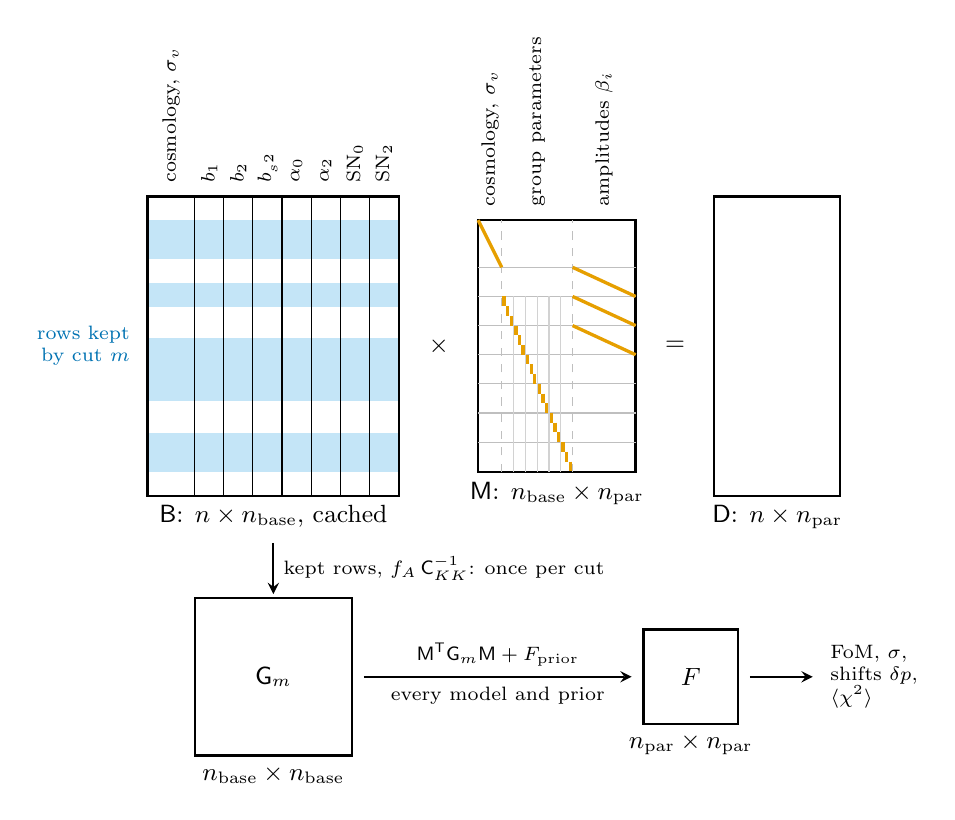
\begin{tikzpicture}[x=1cm, y=1cm, font=\small, >=stealth]
    % --- the base matrix B (n x n_base); shaded rows: one cut
    \foreach \ya/\yb in {0.3/0.8, 1.2/2.0, 2.4/2.7, 3.0/3.5}
      \fill[oksky!35] (0,\ya) rectangle (3.2,\yb);
    \draw[thick] (0,0) rectangle (3.2,3.8);
    \foreach \x in {0.6,0.97,1.34,1.71,2.08,2.45,2.82}
      \draw (\x,0) -- (\x,3.8);
    \node[rotate=90, anchor=west, font=\scriptsize] at (0.3,3.85)
      {cosmology, $\sigma_v$};
    \foreach \x/\l in {0.785/$b_1$, 1.155/$b_2$, 1.525/$b_{s^2}$,
        1.895/$\alpha_0$, 2.265/$\alpha_2$, 2.635/$\SNz$, 3.005/$\SNt$}
      \node[rotate=90, anchor=west, font=\scriptsize] at (\x,3.85) {\l};
    \node[anchor=east, align=right, font=\scriptsize, text=okblue]
      at (-0.1,1.9) {rows kept\\by cut $m$};
    \node[below] at (1.6,0) {$\mB$: $n \times \nbase$, cached};
    % --- times the model M (n_base x n_par); its rows are B's columns
    \node at (3.7,1.9) {$\times$};
    \draw[thick] (4.2,0.3) rectangle (6.2,3.5);
    \foreach \u in {0.6,0.97,1.34,1.71,2.08,2.45,2.82}
      \draw[gray!50] (4.2,3.5-\u) -- (6.2,3.5-\u);
    \draw[gray!50, dashed] (4.5,0.3) -- (4.5,3.5);
    \draw[gray!50, dashed] (5.4,0.3) -- (5.4,3.5);
    % one column range per family of group parameters
    \foreach \k in {1,...,5}
      \draw[gray!35] ({4.5 + \k*0.15},0.3) -- ({4.5 + \k*0.15},2.53);
    % identity on the cosmology and sigma_v
    \draw[okorange, very thick] (4.2,3.5) -- (4.5,2.9);
    % one staircase per family of group parameters (three groups drawn)
    \foreach \k/\top in {0/2.53, 1/2.16, 2/1.79, 3/1.42, 4/1.05, 5/0.68}
      \foreach \j in {0,1,2}
        \draw[okorange, very thick]
          ({4.5 + \k*0.15 + 0.03 + \j*0.045}, {\top - \j*0.1233})
          -- ++(0,-0.1233);
    % the per-bin amplitudes: three diagonals (the chain rule)
    \draw[okorange, very thick] (5.4,2.9) -- (6.2,2.53);
    \draw[okorange, very thick] (5.4,2.53) -- (6.2,2.16);
    \draw[okorange, very thick] (5.4,2.16) -- (6.2,1.79);
    \node[rotate=90, anchor=west, font=\scriptsize] at (4.35,3.55)
      {cosmology, $\sigma_v$};
    \node[rotate=90, anchor=west, font=\scriptsize] at (4.95,3.55)
      {group parameters};
    \node[rotate=90, anchor=west, font=\scriptsize] at (5.8,3.55)
      {amplitudes $\beta_i$};
    \node[below] at (5.2,0.3) {$\mM$: $\nbase \times \npar$};
    % --- equals the model's derivatives D (n x n_par)
    \node at (6.7,1.9) {$=$};
    \draw[thick] (7.2,0) rectangle (8.8,3.8);
    \node[below] at (8.0,0) {$\mD$: $n \times \npar$};
    % --- the cut reduced once to G_m, then every model and prior
    \draw[->, thick] (1.6,-0.6) -- (1.6,-1.25)
      node[midway, right, font=\scriptsize]
      {kept rows, $f_A\,\Cov_{KK}^{-1}$: once per cut};
    \draw[thick] (0.6,-3.3) rectangle (2.6,-1.3);
    \node at (1.6,-2.3) {$\mG_m$};
    \node[below] at (1.6,-3.3) {$\nbase \times \nbase$};
    \draw[->, thick] (2.75,-2.3) -- (6.15,-2.3)
      node[midway, above, font=\scriptsize]
      {$\mM\T \mG_m \mM + F_{\rm prior}$}
      node[midway, below, font=\scriptsize] {every model and prior};
    \draw[thick] (6.3,-2.9) rectangle (7.5,-1.7);
    \node at (6.9,-2.3) {$F$};
    \node[below] at (6.9,-2.9) {$\npar \times \npar$};
    \draw[->, thick] (7.65,-2.3) -- (8.45,-2.3);
    \node[anchor=west, align=left, font=\scriptsize] at (8.55,-2.3)
      {FoM, $\sigma$,\\ shifts $\delta p$,\\ $\langle\chi^2\rangle$};
  \end{tikzpicture}
  \caption{How the notebooks assemble a Fisher matrix.  Top: a model is
    a matrix $\mM$ on the cached base columns $\mB$, and $\mD = \mB\mM$
    are its derivatives.  Orange: the nonzero entries of $\mM$, which
    are the identity on the cosmology and $\sigma_v$, one staircase per
    family of group parameters (ones on the bins of each group; three
    groups drawn), and three diagonals for the per-bin amplitudes
    $\beta_i$ (the chain rule).  Bottom: a cut keeps some rows of $\mB$
    (shaded) and is reduced once to $\mG_m$; every model and prior at
    that cut is then $\mM\T\mG_m\mM$ plus priors.  The check column of
    $\mB$ is not drawn.}
  \label{fig:schematic}
\end{figure}

\section{A scale cut is a set of rows}
\label{sec:cuts}

A cut at $\kmax$, quoted at $z = 0$, cuts bin $i$ at $\kmax/D(\bar{z}_i)$
by the non-Limber ultraviolet-fraction criterion of Saraivanov et
al.~\cite{Saraivanov2026}, within the shipped mask: a band is kept while
less than $5\%$ of it comes from the power spectrum above that
wavenumber.  The cut changes no derivative; it selects the set $K_m$ of
rows that cut $m$ keeps.  With $\mB_K$ the kept rows of $\mB$ and
$\Cov_{KK}$ the kept block of the covariance,
\begin{equation}
  \mG_m \;=\; f_A\, \mB_K\T\, \Cov_{KK}^{-1}\, \mB_K
  \label{eq:gram}
\end{equation}
is an $\nbase \times \nbase$ matrix that holds everything the data of
cut $m$ say about the base columns.  The notebooks compute it once per
cut (\texttt{layout\us grams}): they factorize $\Cov_{KK} = L L\T$ with
$L$ lower triangular (the Cholesky factorization), solve
$W = L^{-1}\mB_K$ by forward substitution, and form
$\mG_m = f_A\, W\T W$.  The inverse covariance is never formed, which
saves work and avoids amplifying round-off on an ill-conditioned
block, and $\mG_m$ is symmetric and positive semidefinite by
construction.  Each layout gets eight such matrices: the seven cuts
$\kmax = 0.05, 0.075, \ldots, 0.2\hMpc$, and the shipped mask alone,
the reference of the information test below.  With
Eq.~\eqref{eq:dbm}, the data part of the Fisher matrix of any model at
any cut is
\begin{equation}
  F_{\rm data} \;=\; \mD_K\T\, f_A\,\Cov_{KK}^{-1}\, \mD_K
  \;=\; \mM\T\, \mG_m\, \mM .
  \label{eq:fdata}
\end{equation}
The model A notebook, which works at one cut, forms $\mD = \mB\mM$
explicitly and multiplies it by the inverse of the kept covariance
block; the two routes agree (Section~\ref{sec:limits}).

\paragraph{The priors.}
$F_{\rm prior}$ adds precision and needs no data.  The diagonal
Gaussian priors, all centered on zero, sit on $\sigma_v$ (from the
example yaml) and on the model's group parameters; the counterterm
widths, $0.5/\kmax^2$, change with the cut, so the diagonal is rebuilt
for each cut (\texttt{prior\us diagonal}).  The linear-bias prior acts
on the block of the $\beta_i$: the baseline and pessimistic priors add
the projected precision of the memory model, group by group
(\texttt{group\us bias\us precision}; the correlated-prior note,
sections ``What the prior charges'' and ``How the prior enters the
Fisher matrix''), the free prior adds nothing, and the growth-tied
prior is a change of $\mM$.

\paragraph{Parameters without data.}
At small cuts some bins keep no band, and their columns vanish on
$K_m$.  A parameter whose information at the cut, data plus prior,
falls below $10^{-10}$ of its information on the shipped mask with the
same priors leaves the fit; a Gaussian prior keeps it in.  A cut that
keeps no band (as $\Delta z = 0.02$ at $\kmax = 0.05\hMpc$) or leaves a
cosmological parameter without data gives no fit.

\paragraph{The pseudo-inverse.}
A plain inverse fails in one more case.  On
$\Delta d_{\rm com} = 62$~Mpc at $\kmax = 0.075\hMpc$ only $7$ of the
$18$ BGS bins keep a band, and under model A + tilts on the free prior
the flat-prior BGS tilts leave one combination of parameters with no
information at all.  Along such a direction a plain inverse amplifies
round-off by about $10^{16}$; it once produced a spurious $2\sigma$
shift.  \texttt{stable\us inverse} therefore scales $F$ to unit
diagonal, $\tilde{F} = S F S$ with $S = {\rm diag}(F)^{-1/2}$, so that
the parameters' units do not matter, diagonalizes
$\tilde{F} = V \Lambda V\T$, drops the directions whose eigenvalue is
below $10^{-12}$ of the largest, and returns
\begin{equation}
  F^{-1} \;=\; S\, V_\kappa\, \Lambda_\kappa^{-1}\, V_\kappa\T\, S ,
  \label{eq:pinv}
\end{equation}
with $\kappa$ the kept directions.  A dropped direction must leave
$(w_0, w_a)$, $\Omega_m$ and $A_s$ alone: the scan gives no fit when one
touches them by more than $10^{-6}$.

\section{Everything downstream reuses $\mG$}
\label{sec:downstream}

Once $\mG_m$ is built, nothing in the notebooks touches an $n \times n$
matrix or the likelihood again.  $F$ is Eq.~\eqref{eq:fdata} plus the
priors, inverted by Eq.~\eqref{eq:pinv}, and $\sigma_j$ and the FoMs
follow as in Section~\ref{sec:linear}.

\paragraph{Shifts.}
A truth that departs from the fitted model moves the data by $\delta m$.
When $\delta m$ lies in the span of the base columns, $\delta m = \mB c$
with $c$ a vector of $\nbase$ coefficients: $\alpha_2 = 12.5\aunit$ in
every bin is $c = 12.5$ on the $\alpha_2$ block, an offset truth puts
its values on the $b_2$ and $\bstwo$ blocks, and a fractional drift $\delta_i$ of the
linear biases is $c = \sum_i \beta_i\,\delta_i\, \mM_{\beta_i}$, with
$\mM_{\beta_i}$ the column of Eq.~\eqref{eq:chain}.  To first order the
fit moves by
\begin{equation}
  \delta p \;=\; F^{-1} \mD\T \Cov^{-1} \delta m
  \;=\; F^{-1} \mM\T\, \mG_m\, c
  \label{eq:shift}
\end{equation}
(the correlated-prior note, ``The shift formula'').  $\delta m = \mB c$
is exact for the $\alpha_2$, $\SNz$ and $\SNt$ truths, whose terms are
linear, and first order for truths in $b_1$, $b_2$ and $\bstwo$, since
the band powers are quadratic in the biases.  A truth costs one product
with $\mG_m$.

\paragraph{Random truths.}
Eq.~\eqref{eq:shift} is linear in $c$, so a family of random truths
collapses into one matrix: for drifts $\delta_i$ of the linear biases
the $(w_0, w_a)$ shift is $\delta w = A\,\delta$, with $A$ the
$(w_0, w_a)$ rows of Eq.~\eqref{eq:shift} applied to the $N$ columns
$\beta_i \mM_{\beta_i}$.  Two thousand truths cost one matrix product.

\paragraph{The exact $\langle\chi^2\rangle$.}
Whether a fit's error bars are honest is tested by averaging
$\chi^2_w = (\hat{w} - w_{\rm true})\T \Cov_w^{-1}
(\hat{w} - w_{\rm true})$, with $\hat{w}$ the fitted $(w_0, w_a)$,
over the truths and the data noise.  Every source is Gaussian and
enters linearly, so the average is exact in closed form (the
correlated-prior note, ``The test statistic''):
\begin{equation}
  \langle \chi^2_w \rangle \;=\; \Delta_{\rm drift}^2
  \;+\; {\rm tr}\!\left[\Cov_w^{-1}\left(A\,\Sigma\,A\T
    + R\,\Sigma_\theta\,R\T + N_w\right)\right] .
  \label{eq:chi2}
\end{equation}
Here $\Delta_{\rm drift}$ is the $(w_0, w_a)$ shift of the known drift
alone, in units of the ellipse; $\Sigma$ the covariance of the truth's
linear-bias residuals; $R$ and $\Sigma_\theta$ the response to, and the
prior variance of, any other parameter drawn at random ($\alpha_2$ per
group in the random test of model B); and $N_w$ the $(w_0, w_a)$ block
of $F^{-1}F_0F^{-1}$, the share of the data noise and the Gaussian
priors, with $F_0$ the Fisher matrix without the linear-bias
precision.  The notebooks report $\chidof$, with $n_{\rm dof} = 2$ for
$(w_0, w_a)$, and $n_{\rm dof} = 1$ for $\Omega_m$ or $A_s$ with that
parameter's own row; $1$ means honest error bars.  The random draws
only make the percentile bars of the figures.

\paragraph{The cost.}
Each $\mG_m$ costs one Cholesky factorization of at most $7{,}621$
rows, about $n_K^3/3 \approx 1.5\times10^{11}$ floating-point
operations, and one triangular solve, eight times per layout.  A Fisher
system then costs $\mM\T\mG_m\mM$, with $\nbase \le 645$ and
$\npar \le 164$ (model B + tilts on $\Delta z = 0.02$), about
$2\,\nbase^2 \npar \approx 1.4\times10^{8}$ operations, plus the
diagonalization of an $\npar \times \npar$ matrix: a fraction of a
second.  The $\kmax$ scan of the model B notebook has $336$ systems
(four layouts, seven cuts, four variants, and the baseline,
pessimistic and free priors; the growth-tied prior fails the accuracy
test and is left out), $324$ with a fit and $12$ without any band.  In
operations, all of them together cost less than the Cholesky
factorizations of one layout.  Without the decomposition, each variant
would need its own derivatives, at the cost of
Section~\ref{sec:holds} per layout, and each truth its own data
vector.

\section{Limits and checks}
\label{sec:limits}

\paragraph{What needs new likelihood evaluations.}
\begin{itemize}
  \item \textbf{A physical term outside the span of $\mB$.}  A term
    that is no combination of the per-bin operators and templates,
    such as a nonzero third-order bias $b_3$ or redshift-space one-loop
    terms (which CosmoLike lacks), needs new base columns.  A new
    combination of existing operators, such as a quadratic tilt or
    another calibration slope at the same fiducial values, is only a
    new $\mM$.
  \item \textbf{A different fiducial point.}  Every derivative is taken
    at $p_0$.  A new fiducial cosmology, new fiducial biases, or a
    calibration law that moves the fiducial $b_2$ needs new base
    columns, and a new covariance, which sits at the one-loop fiducial.
    A new covariance alone needs no likelihood evaluation: the
    notebooks rebuild every $\mG_m$ from the current covariance file at
    every run.
  \item \textbf{Dependence beyond first order.}  The forecast is the
    curvature at $p_0$, and Eq.~\eqref{eq:shift} is first order in
    $\delta m$.  The band powers are quadratic in the biases, so a large
    truth, such as an offset of twice a prior width or the $22\%$ BGS
    flux-limit drift, is treated to first order, and a shift near the
    $\sigma/3$ threshold needs a refit, with new evaluations, to be
    confirmed.
\end{itemize}

\paragraph{The checks that guard the machinery.}
\begin{itemize}
  \item \textbf{The chain rule.}  The per-bin columns, obtained through
    the intercepted setter and summed over a group,
    $\sum_{i \in g} \partial m/\partial \beta_i$ with
    Eq.~\eqref{eq:chain}, must equal the stencil derivative
    $\partial m/\partial B_g$, obtained through the full likelihood.
    The two routes share no evaluation; they agree to
    $1.2\times10^{-7}$ of the stencil column's largest entry (the
    correlated-prior note, ``Numerical checks'').
  \item \textbf{Bitwise template checks.}  The order-$0$ templates of a
    template run must equal the cached $\SNz$ templates exactly, and the
    run's fiducial vector the cached one.  $\mB$ carries the difference
    of the two vectors as its check column, so their $\Delta\chi^2$ is a
    diagonal entry of $\mG$ on the shipped mask; it is zero.  After the
    $\alpha_2$ steps the vector must equal the one before bit for bit
    (the setter is back at zero), and the forward and backward
    $\alpha_2$ differences must agree (the term is linear).
  \item \textbf{The matched-prior check.}  When the truth's linear-bias
    scatter equals the fit's prior and every other parameter is drawn
    from the fit's own priors, the projected precision $\mathsf{P}$
    obeys $\mathsf{P}\Sigma\mathsf{P} = \mathsf{P}$, and the scatter
    and noise terms of Eq.~\eqref{eq:chi2} add up to exactly
    $n_{\rm dof}$ (the correlated-prior note, ``The test statistic'').
    The notebooks verify this on every system to round-off, which tests
    $\mG$, $\mM$, the priors and the pseudo-inverse together.  The
    model A FoMs of the model B notebook's scan also equal those of the
    model A notebook, assembled by the other route of
    Section~\ref{sec:cuts}, to $7.9\times10^{-10}$, and a $+$ and a $-$
    truth give shifts of equal size.
  \item \textbf{The cache-settings check.}  Each cache stores the
    settings it was computed with, and a notebook refuses a cache whose
    settings differ from its own (Section~\ref{sec:usage}).
\end{itemize}

\section{Using the caches}
\label{sec:usage}

The caches live in \texttt{chains/}, which git ignores: a fresh clone
recomputes them (hours), and every later run reads them.  Their names
start with \texttt{EXAMPLE\us EVALUATE\us FISHER}, and
$\langle n\rangle = 1$ to $4$ numbers the layouts in the order
$\Delta d_{\rm com} = 62$~Mpc, $\Delta z = 0.02$, $0.05$, $0.2$.
\begin{itemize}
  \item \texttt{\us SCALE\us CUTS.pkl}, written by the linear notebook,
    \texttt{EXAMPLE\us EVALUATE\us FISHER.ipynb}: the bands each
    ultraviolet-fraction cut keeps, at
    $\kmax = 0.05, 0.075, \ldots, 0.25\hMpc$; the scans use the seven
    cuts up to $0.2$.
  \item \texttt{\us MODEL\us A\us DERIVATIVES\us<n>.pkl}, written by the
    model A notebook,
    \texttt{EXAMPLE\us EVALUATE\us FISHER\us MODEL\us A.ipynb}, flag
    \texttt{RECOMPUTE}: the fiducial point and vector, the $20$ stencil
    columns, the per-bin columns of $b_1$, $b_2$, $\bstwo$ and
    $\alpha_0$, the $\SNz$ templates, the fiducial per-bin biases, the
    group of each bin, the Gaussian prior widths and the settings.
  \item \texttt{\us MODEL\us A\us SN2\us<n>.pkl}, model A notebook, flag
    \texttt{RECOMPUTE\us SN2}: the $\SNt$ templates, kept apart so that
    the derivative caches stay as they are.
  \item \texttt{\us MODEL\us B\us TEMPLATES\us<n>.pkl}, written by the
    model B notebook,
    \texttt{EXAMPLE\us EVALUATE\us FISHER\us MODEL\us B.ipynb}, flag
    \texttt{RECOMPUTE\us TEMPLATES}: the $\alpha_2$ columns and the
    $\SNz$ and $\SNt$ templates.
\end{itemize}
The model A and B notebooks cache no Fisher matrix, $\mG_m$ or FoM:
these depend on the covariance and are rebuilt at every run.

\paragraph{The flags.}
With a flag at \texttt{False}, the default, a notebook reads an
existing cache after the settings check and computes a missing one;
\texttt{True} recomputes it and overwrites the file.  The layouts are
computed cheapest first, and each cache is written as soon as its
layout is done, so an interrupted run keeps the finished layouts.  The
model B notebook reads the model A caches and never writes them; it
stops when one is missing or was made with other settings.  For a
fresh clone, run the linear notebook (for the cuts), then the model A
notebook, then the model B notebook.

\paragraph{What invalidates a cache.}
\begin{itemize}
  \item \textbf{Detected automatically}: a change of the stored
    settings, which are the example yaml and the parameter file
    (compared by file name, so a moved file keeps its cache), the
    dataset, the likelihood overrides, the accuracy settings and the
    steps.  The notebook stops and asks for the flag.
  \item \textbf{Not detected, so set the flag by hand}: a change of the
    code (the likelihood, CosmoLike, CAMB), or of the content of a yaml
    or parameter file under the same name (the fiducial point, the
    grouping, an accuracy option).  No check compares a cache with the
    current code unless a cache is recomputed; the fiducial-vector
    check then catches a change that moves the fiducial vector.
  \item \textbf{Needs no recomputation}: a new covariance, a new prior
    or prior width, a new model built from the cached operators, and
    any cut already in the cut cache.  A $\kmax$ outside it needs the
    linear notebook to compute that cut (CosmoLike's split of each band
    into the power below and above the cut), but no new derivative.
\end{itemize}

\begin{thebibliography}{99}

\bibitem{Lazeyras2016}
T. Lazeyras, C. Wagner, T. Baldauf and F. Schmidt,
``Precision measurement of the local bias of dark matter halos'',
2016, arXiv:1511.01096.

\bibitem{Saraivanov2026}
E. Saraivanov, H. Rubira, V. Miranda and T. Eifler,
``Towards the Two-Loop EFTofLSS in Galaxy Lensing Surveys'',
2026, arXiv:2603.13031.

\end{thebibliography}

\end{document}
